%This is for the neutrino mass measurements


\section{Determination of neutrino mass and nature}

The absolute values of neutrino masses and the neutrino nature (Dirac versus Majorana) are among the most fundamental open questions in physics today. The determination of these neutrino properties will be an essential ingredient to understand the origin of neutrino mass, and the role of neutrinos in the universe. Due to their abundance and their being initially relativistic, neutrinos play a crucial role in large-scale structure formation of the universe. Their potential Majorana nature would be a key to solve the puzzle of the matter-antimatter asymmetry of the universe. 

\subsection{Cosmology}
Cosmological observations themselves provide powerful probes of the neutrinos mass. They are mainly based on the fact that neutrinos, due to their relativistic velocities and large free-streaming lengths, prevent the formation of small-scale structures in early epochs of the universe. Current limits based on the Planck satellite set limits of $m_{\nu} = \sum_i m_{\nu_i}<230 - 540$~meV (95\% CL)~\cite{Aghanim:2018eyx}. Future surveys, such as the imaging and spectroscopic space telescope EUCLID~\cite{Laureijs:2011gra} (to be launched in 2022 for a six years mission), aim for the first time at an actual measurement of the neutrino mass with a precision of $\sigma({m_{\nu} }) = 10$~meV. %It is important to note, however, that these results will depend on the precise knowledge of other cosmological parameters, such as the so-called optical depth and the underlying cosmological model~\cite{Boyle:2017lzt, Boyle:2018rva}.
%TSM:
It is important to note however that, despite their sensitivity, these results will depend on the underlying cosmological model, and could be affected by degeneracies with other cosmological parameters~\cite{Boyle:2017lzt, Boyle:2018rva}.  This stresses the importance of performing the measurement of the absolute neutrino masses both via cosmological observables and with the even more challenging direct methods. A good agreement between these two approaches would be a crowning confirmation of the cosmological model.


\subsection{Neutrinoless double beta decay}

The search for neutrinoless-double $\beta$-decay ($0\nu\beta\beta$) is a unique probe of the nature of neutrinos. Discovering this process
would indeed prove that neutrinos are Majorana particles and hence that Lepton number is violated in nature. 
This discovery would in addition provide insight into the absolute neutrino mass scale.

The half-life for this process $T_{1/2}$ is inversely proportional to the square of the Majorana neutrino
mass $m_{\beta \beta}= | \sum_i  U^2_{ei} m_i |$. The predictions for $m_{\beta \beta}$ depend on the neutrino mass spectrum. For the inverted ordering there is a lower bound of 15 meV, while for the normal one $m_{\beta \beta}$ can go from the current bounds to zero, for specific values of the neutrino masses. Apart from light Majorana neutrinos, other lepton number violating mechanisms can mediate this process.


The current best neutrino mass limit of $m_{\beta\beta} = 50 - 160$~meV is provided by the KamLand Zen experiment~\cite{KamLAND-Zen:2016pfg} in Japan. The best half-life sensitivity of $T_{1/2}>11\times 10^{25}$ years (90\% CL) was achieved by the \textsc{Gerda} experiment~\cite{zsigmond} (LNGS, Italy). Thanks to their scalability, future $0\nu\beta\beta$ experiments plan to reach sensitivities down to $m_{\beta\beta} \approx 10$~meV, covering the allowed parameter space for inverted neutrino mass ordering (Fig.~\ref{fig:doublebeta}). 
%Even if normal ordering is realized in nature, their discovery sensitivity still reaches about 50\%~\cite{Agostini:2017jim, Caldwell:2017mqu}. 
%TSM: not convinced by this type of argument - very prior/analysis dependent!

\begin{figure} [htbp!]
\begin{center}
%add plot!!!
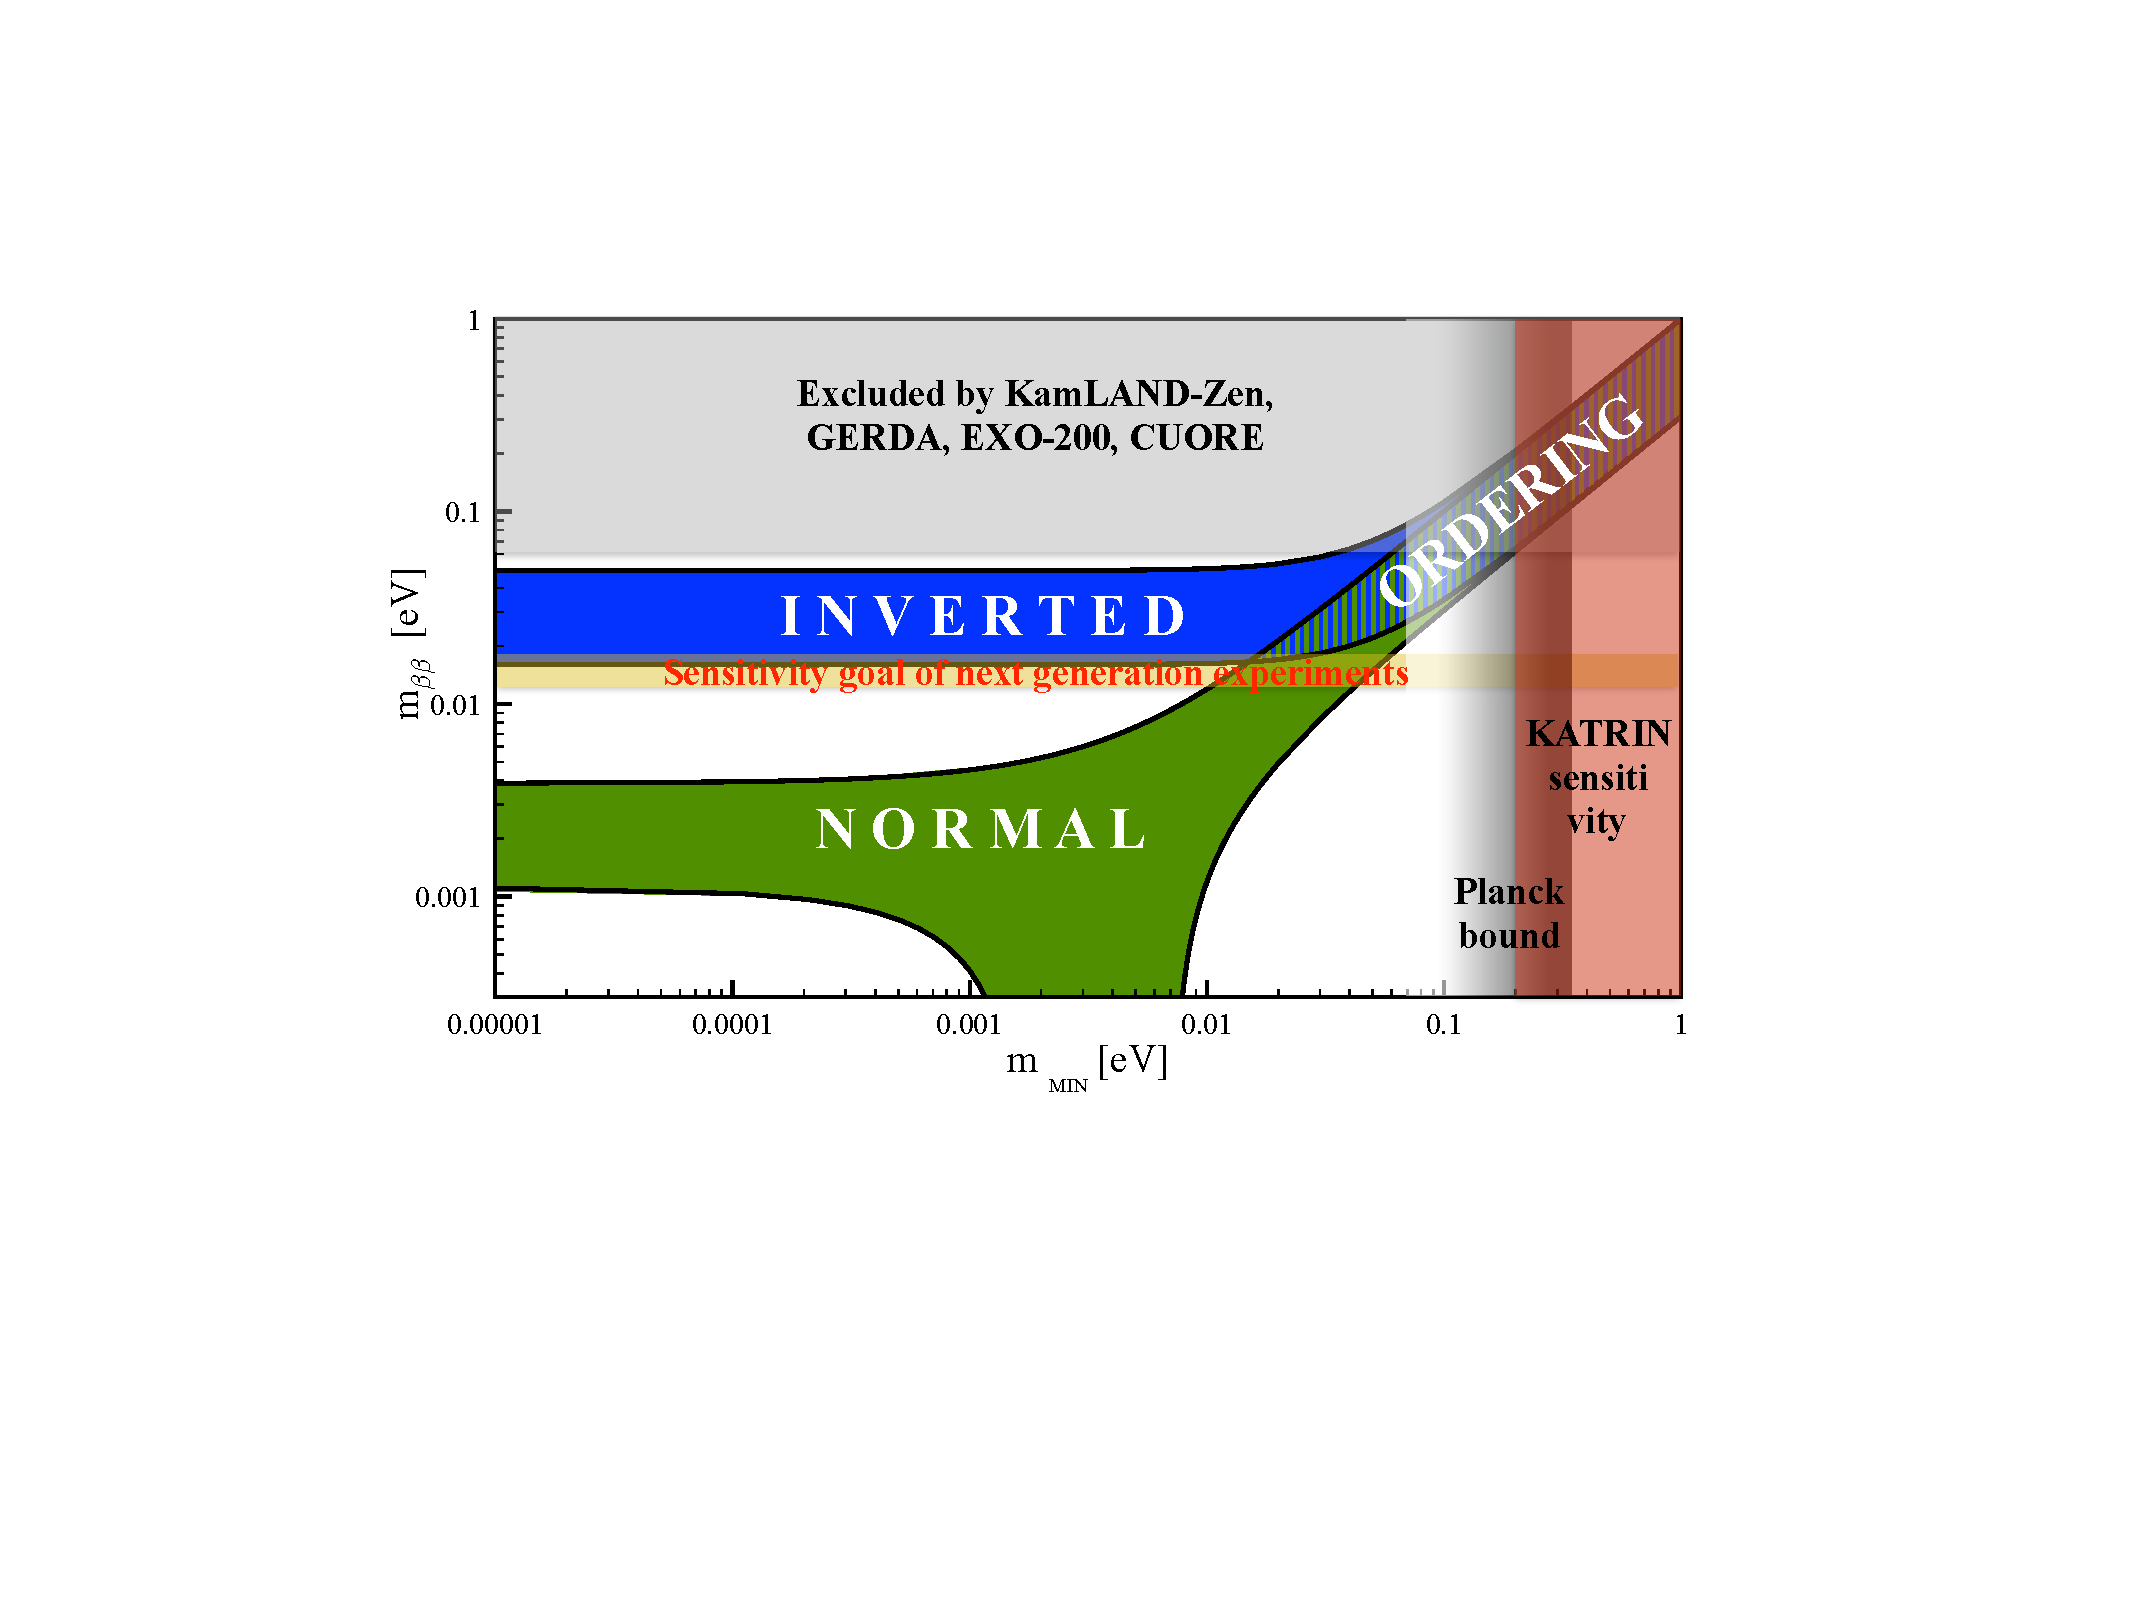
\includegraphics[width=14cm]{\main/Neutrino/img/doublebetaplot.pdf}
\caption{\label{fig:doublebeta} 
The effective mass $ m_{\beta \beta}$ controlling the rate of the neutrino-less double beta decay versus the mass of the lightest eigenstate\cite{pascoli}. The limits from the current and future experiments are shown.}
\end{center}
\end{figure}


The European roadmap for this experimental program is presently being developed under the aegis of APPEC.
The next-generation LEGEND experiment~\cite{DAndrea:2019umy}, successor of the \textsc{Gerda}~\cite{Agostini:2018tnm} and \textsc{Majorana}~\cite{Aalseth:2017btx, Alvis:2019sil} experiments, targets to operate 1000~kg of Ge-semiconductor detectors (enriched in ${}^{76}$Ge) to reach a 3$\sigma$ discovery sensitivity of $>10^{28}$~years, corresponding to a mass limit of $m_{\beta\beta} < 10 - 17 $~meV. The nEXO experiment~\cite{Albert:2017hjq}, successor of EXO~\cite{Albert:2017owj}, plans to instrument a 5-tonne liquid xenon (enriched in ${}^{136}$Xe) time projection chamber to reach a 3$\sigma$ discovery sensitivity of $5.6\times 10^{27}$~years, corresponding to a mass limit of $m_{\beta\beta} < 5.7 - 17.7$~meV. NEXT~\cite{Alvarez:2011my} explores an alternative approach based on gaseous xenon TPC, which has advantageous features both with respect to energy resolution and background suppression. It is interesting to note, that also future xenon-based dark matter experiments, such as DARWIN~\cite{Aalbers:2016jon}, may have competitive sensitivity to $0\nu\beta\beta$. The next-generation CUPID experiment~\cite{Azzolini:2018tum}, the successor of CUORE~\cite{Alduino:2017ehq}, plans to employ cryogenic detectors, which allow for both heat and light signal readout. Promising results have been obtained with $^{130}$TeO$_{2}$~\cite{Artusa:2016mat}, Zn$^{82}$Se~\cite{Azzolini:2018dyb}, Li$_2^{100}$MoO$_4$~\cite{Bekker:2014tfa} crystals. %The latter depicts the baseline for a future large-scale experiment. 

\subsection{Direct neutrino mass experiments}
The least model-dependent technique to determine the absolute neutrino mass scale is based on the kinematics of single-$\beta$-decay~\cite{Drex13}. Here, the impact of the so-called effective electron (anti-)neutrino mass $m^2_{\nu_e}  = \sum_i |U_{ei}|^2 m_{\nu_i}^2$ is a reduction of the kinematic endpoint energy $E_0$ and a distortion of the beta-decay spectrum close to this endpoint. 

Single-beta-decay experiments are also ideally suited to perform searches for eV- to keV-scale sterile neutrino searches. These hypothetical neutrinos would manifest themselves as spectral distortion at an energy $E = E_0 - m_s$, where $m_s$ is the mass of the sterile neutrino. These searches are highly complementary to oscillation-based searches~\cite{Boser:2019rta, Mer:2015a}. 

The Karlsruhe Tritium Neutrino (KATRIN) experiment, a large-scale tritium beta decay experiment~\cite{Angrik:2005ep}, started data taking in 2019. KATRIN combines an ultra-luminous gaseous tritium source ($10^{11}$ decays per second) with a high-resolution magnetic-adiabatic collimation and electrostatic filter~\cite{Otten:2008zz,Lobashev:1985mu, PICARD1992345}. The design sensitivity of 200~meV (90\% CL) will be reached after 5 calender years of data taking. 

A complementary approach is pursued by the ECHo~\cite{Gastaldo:2017edk} and Holmes~\cite{Giachero:2016xnn} experiments, which exploit the electron-capture decay of $^{163}$Ho. New ideas based on cyclotron emission spectroscopy (CRES) and the usage of atomic tritium are being explored by the Project-8 experiment~\cite{Esfahani:2017dmu} to push the sensitivity beyond the degenerate mass regime to about 40~meV (90\% CL).

